\documentclass[a4paper,10pt,openright,openbib,twocolumn]{article}
%\usepackage[portuges]{babel}
\usepackage[T1]{fontenc}
\usepackage{ae}
\usepackage[utf8]{inputenc}
\usepackage[pdftex]{graphicx}
\usepackage{url}
\usepackage{listings}
\usepackage{verbatim}
\usepackage{enumerate}
\usepackage[pdftex, bookmarks, colorlinks, linkcolor=black, urlcolor=blue]{hyperref} 
\usepackage[a4paper,left=2.5cm,right=2.5cm,top=3.5cm,bottom=3.5cm]{geometry}
\usepackage{colortbl}
\usepackage[margin=10pt,font=small,labelfont=bf]{caption}
\usepackage{mdwlist}
\usepackage{cleveref}
\usepackage{epsfig}

\usepackage{multicol}
\usepackage{appendix}
\usepackage{float}

\setlength{\parindent}{0cm}
\setlength{\parskip}{2pt}


\begin{document}

\begin{multicols}{2}
\title{Parallel Simulated Annealing Algorithm Study}
\author{
    Brito, Rui\\
    PG22781\\
    Department of Informatics\\
    University of Minho\\
    ruibrito666@gmail.com
  \and
    Alves, José\\
    PG22765\\
    Department of Informatics\\
    University of Minho\\
    zealves.080@gmail.com
}
\date{}
\maketitle
\end{multicols}

\begin{abstract}

\end{abstract}

\section{Introduction}
In this report we present a study of a Parallel Simulated Annealing algorithm for solving the room assignment problem. Simulated annealing is an interative method based on the process of physical annealing.
This algorithm starts by choosing a solution wich might be worse than a solution given by a probability function. In each iteration it decrease the probability of a worse solution, closing the gap from a local limited solution to a more global and optimized one.

This project compares two algorithms for resolving the Room Assignment problem, one with Simulated Annealing and one without. The algorithms were both implemented in sequential and openMPI, in C. Both versions were tested with the same matrix of incompability values from a range of pseudo-generated values.

This reports study the result of the simulated annealing method in a Room Assignment problem, studying the variation of parameters and the results obtained

This report starts with a brief Introduction followed by a Case Study section where the problem is explained. The Algorithm section shows the implementation of said algorithm and some reasoning behind some decisions. We then present the results, comparing both versions of the algorithm in the section Results. Finally a brief conclusion summarizes the project in the last section of the report.

\section{Case Study}

The Case Study here presented is the Room Assignment Problem. This is a problem of optimization where the simulated annealing gives better solutions than a regular probablistic algorithm.

The problem consists in assigning students($n$) to rooms($\frac{n}{2}$), but minimizing the conflits between roomates.

The objective of this case study is to minimize the cost of the distribution. Since the magnitude of the problem is very big and there is no way of analysing all possible states in a acceptable amount of time, we use simulated annealing. Using this mehod we can make a good aproximation of the optimal value with less computation.

To start a pseudo-random matrix is created to represent the room distribution. For each iteration two randomly selected students and exchanged, if the cost is lower in the new matrix-state the change is made, if not it is reversed.
The conflits are registered in a matrix, where it shows how many students have conflits with each other.
The current cost of a state is equal do the sum of all conflits.

The method sets a high temperature for the system, making the first iterations more disperse and random. While the temperature of the system lowers with each iteration, the result starts to approach a better solution, finding a better global solution with lower cost.

The method of simulated annealing modifies the conditions of how the swap is taken. Using simmulated annealing the system considers the difference between the state before the swap and after the swap. Without simulated annealing only states with lower cost are accepted making the solution more narrow and local.

\section{Algorithm}
The program developed have a sequential version and a distributed memory version. 
The first part of the algorithm maintains the same structure, first selecting both students who are not roomates, find their respective rooms and calculating their conflit ratio.

\begin{verbatim}
(...)
//Select students
s1 = randomul_limited(0, laststudent);
s2 = randomul_limited(0, laststudent);
(...)

// Room of the first student
r1 = assigned[s1];
sa = rooms[r1 * 2    ];
sb = rooms[r1 * 2 + 1];
p1 = (s1 == sa);
s3 = p1 ? sb : sa;

// Room of the second student
r2 = assigned[s2];
sa = rooms[r2 * 2    ];
sb = rooms[r2 * 2 + 1];
p2 = (s2 == sa);
s4 = p2 ? sb : sa;

// Conflit coeficient
dcost = dislikes[s1 * nstudents + s4]
              + dislikes[s2 * nstudents + s3]
              - dislikes[s1 * nstudents + s3]
              - dislikes[s2 * nstudents + s4];  


\end{verbatim}

In the next step is where the algorithms differ. The algorithm below shows what is done for the version without simulated annealing.

\begin{verbatim}    
        if ( dcost < 0 ) {  
            assigned[s3] = r2;
            assigned[s4] = r1;
            rooms[r1 * 2 + p1] = s4;
            rooms[r2 * 2 + p2] = s3;    
            if (dcost) {
                cost += dcost;
                j = nstudents;
            } else
                --j;
            
            i = max;
        }
        else
        {
            --i;
        }
\end{verbatim}
As we can see above, the algorithm only accept change when the dislike cost of each specific room is lower than before. This turns the solution very local since it doesn't take inconsideration the other rooms.

\begin{verbatim}
        double r = randDouble();
        double f = (double) (- dcost) / (double) t;
        double e = exp(f);

        if (dcost < 0 || (e >= r)) {    
            assigned[s3] = r2;
            assigned[s4] = r1;
            rooms[r1 * 2 + p1] = s4;
            rooms[r2 * 2 + p2] = s3;
    
            if (dcost) {
                cost += dcost;
                j = nstudents;
            } else
                --j;

            if (cost && dcost < 0 && ((unsigned long)(- dcost)) > cost)
                cost = 0;           
            
            i = max;
        }
        else {
            --i;
        }

        //cool the system
            t *= 0.999;
    }

\end{verbatim}

In the simulated annealing version the algorithm compares the swapping cost with the current one, if the swap cost is lower or the temperature is high enough so that $e^{-dcost/T}$ is higher than a randomly generated value, $r$, the swap is accepted and the number of iterations set to zero.    

\section{Results}

First we can observe the results for the !!!!!!!!!!!!! version and the !!!!!!!!!!!!!!!!! version.
\begin{figure}[!htb]
    \centering
    \begin{minipage}[t]{\columnwidth}
        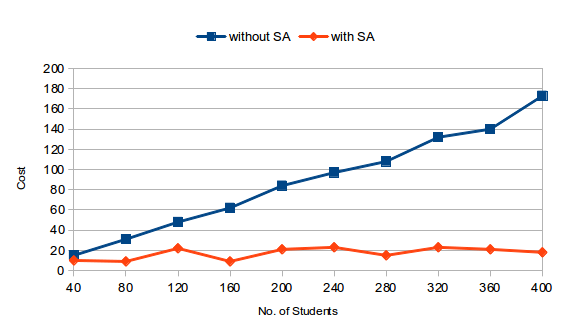
\includegraphics[width=\textwidth]{./img/rand-1.png}
        \caption{ASDASDASD\label{fig:parallel}}
    \end{minipage}
\end{figure}


\begin{figure}[!htb]
    \centering
    \begin{minipage}[t]{\columnwidth}
        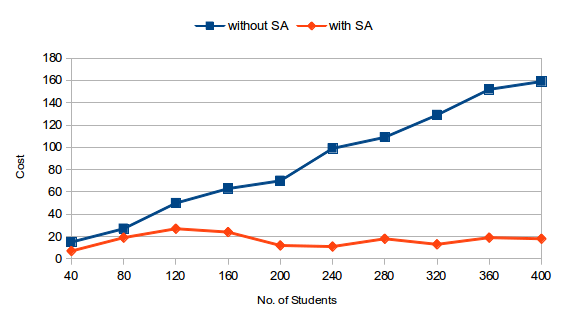
\includegraphics[width=\textwidth]{./img/arc4-1.png}
        \caption{ASDASDASD\label{fig:parallel}}
    \end{minipage}
\end{figure}

Here we can compare the results of both versions.

\begin{figure}[!htb]
    \centering
    \begin{minipage}[t]{\columnwidth}
        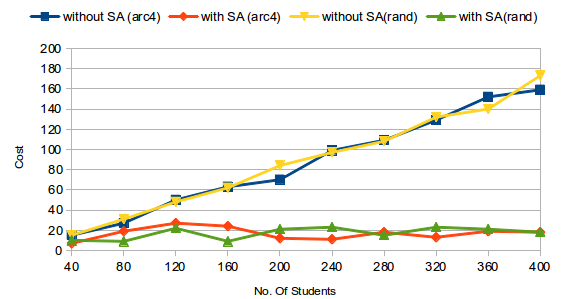
\includegraphics[width=\textwidth]{./img/mix.png}
        \caption{ASDASDASD\label{fig:parallel}}
    \end{minipage}
\end{figure}

As we can see in the picture the !!!!!!!!!!!!!!!!!!!!!!!!!!!!!!.

Next we can see the algorithm working for the difference number of processes.

\begin{figure}[!htb]
    \centering
    \begin{minipage}[t]{\columnwidth}
        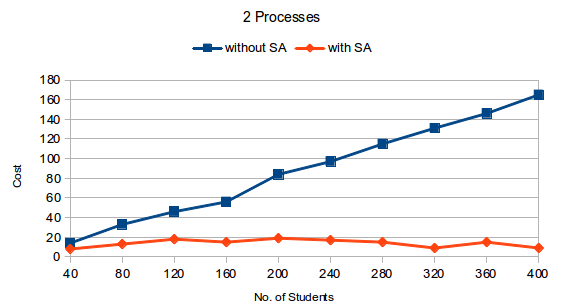
\includegraphics[width=\textwidth]{./img/arc4-2.png}
        \caption{Results for the program in 2 Processes.\label{fig:parallel}}
    \end{minipage}
\end{figure}

\begin{figure}[!htb]
    \centering
    \begin{minipage}[t]{\columnwidth}
        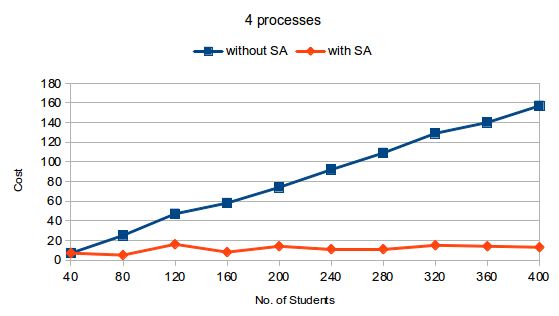
\includegraphics[width=\textwidth]{./img/arc4-4.png}
        \caption{Results for the program in 4 Processes.\label{fig:parallel}}
    \end{minipage}
\end{figure}

As we can see in the results, the final solution is always better for the simulated annealing approach.


\begin{figure}[!htb]
    \centering
    \begin{minipage}[t]{\columnwidth}
        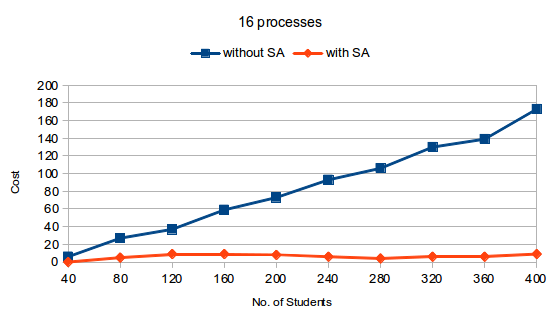
\includegraphics[width=\textwidth]{./img/arc4-16.png}
        \caption{Results for the program in 16 Processes.\label{fig:parallel}}
    \end{minipage}
\end{figure}

\begin{figure}[!htb]
    \centering
    \begin{minipage}[t]{\columnwidth}
        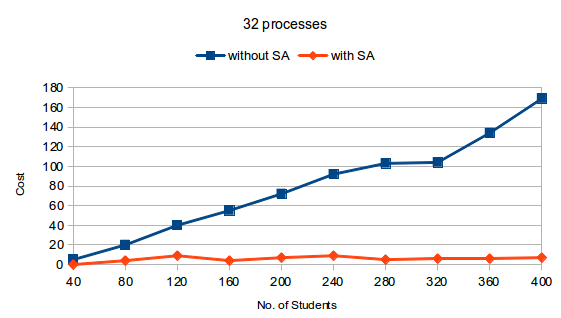
\includegraphics[width=\textwidth]{./img/arc4-32.png}
        \caption{Results for the program in 32 Processes.\label{fig:parallel}}
    \end{minipage}
\end{figure}

The results clearly show a improvement in the solutions when using simulated annealing. Following a worse case solution in the first iterations, led us to find a better overall solutions. Since the algorithm is embarrassingly parallel the cost of parallelizing the program were minimal and provide us with more resources to find a better solution in a similar amount of time. 

\section{Conclusion}

The problem studied in this paper is the Room Assignment problem using simulated annealing method. This method computes a more general and overall low solution by allowing worse solutions while decreasing the overall cost.

As stated above the algorithm is embarrassingly parallel so an approach using distributed memory was created. Since each process can calculate its optimal solution using their pseudo generated numbers, a better result can be achieved by the program.

The final result were objective, showing much better cost for the simulated annealing approach. Allowing the algorithm to follow worse solutions in the beggining, proved to be a good bet in the long run. 

\end{document}
